\documentclass{article}
\usepackage{amsmath}
\usepackage{tikz}
\usetikzlibrary{positioning}

\begin{document}



\textit{Sea \( G \) un digrafo con dos vértices \( s \) y \( t \) Dar un algoritmo que cuente la cantidad de caminos disjuntos en aristas } \\

Construimos una red \( N \) a partir de nuestro digrafo con las siguientes características:
Si existía una arista \( (v, w) \) y \( (w, v) \) en \( G \), creamos el nodo \( v' \) tal que las aristas en la red son \( (v, w) \), \( (w, v') \), \( (v', v) \).

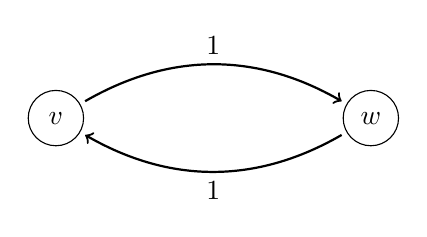
\begin{tikzpicture}[
    vertex/.style={circle, draw, minimum size=20pt, inner sep=0pt},
    edge/.style={->, thick, shorten >=2pt, shorten <=2pt}
  ]
  % Original Digraph G
  \node[vertex] (v) at (0,0) {$v$};
  \node[vertex] (w) at (4,0) {$w$};
  
  \draw[edge] (v) to[bend left] node[above] {$1$} (w);
  \draw[edge] (w) to[bend left] node[below] {$1$} (v);
  
  
\end{tikzpicture}
\hspace{1cm}
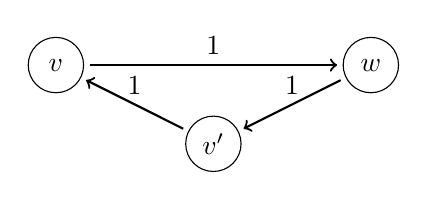
\begin{tikzpicture}[
    vertex/.style={circle, draw, minimum size=20pt, inner sep=0pt},
    edge/.style={->, thick, shorten >=2pt, shorten <=2pt},
    virtual/.style={circle, draw=none, minimum size=20pt, inner sep=0pt, opacity=0.4}
  ]
  % Transformed Network N
  \node[vertex] (v) at (0,0) {$v$};
  \node[vertex] (w) at (4,0) {$w$};
  \node[vertex] (v') at (2,-1) {$v'$};
  
  \draw[edge] (v) to node[above] {$1$} (w);
  \draw[edge] (w) to node[above] {$1$} (v');
  \draw[edge] (v') to node[above] {$1$} (v);
  
  
\end{tikzpicture}




A todas las aristas les damos capacidad 1.

Usamos Edmonds-Karp desde el vértice \( s \) en nuestro modelo. El flujo máximo será igual a la cantidad de caminos disjuntos en aristas.

Pensemos un poco por qué: Al tener cada arista capacidad 1, solo podrá ser "usada" para un camino una sola vez, impidiendo que contemos caminos con una arista repetida. Luego, la cantidad de flujo que llega a \( t \) será equivalente a la cantidad de caminos disjuntos en aristas.

Visto sobre la implementación, cada vez que encontramos un camino de aumento en el grafo residual, sabemos que es un camino donde necesariamente no hay ninguna arista usada (ya que recordemos tenemos capacidad 1). Como el cuello de botella será siempre 1, el flujo representa exactamente la cantidad de caminos.

Complejidad: \( O(mF)) \leq O(m^2) \) (La cantidad de caminos es siempre menor o igual a la cantidad de aristas).

\end{document}
